\section{Risultati}
Questa sezione è deidcata ai risultati sperimentali. L'ultima riga della tabella contiene il rapporto fra il tempo di PDIP-LDL e QUADPROG.
\subsection*{subexp 1}

Qua no ho capito un cazo 

\begin{figure}[!h]
    \centering
    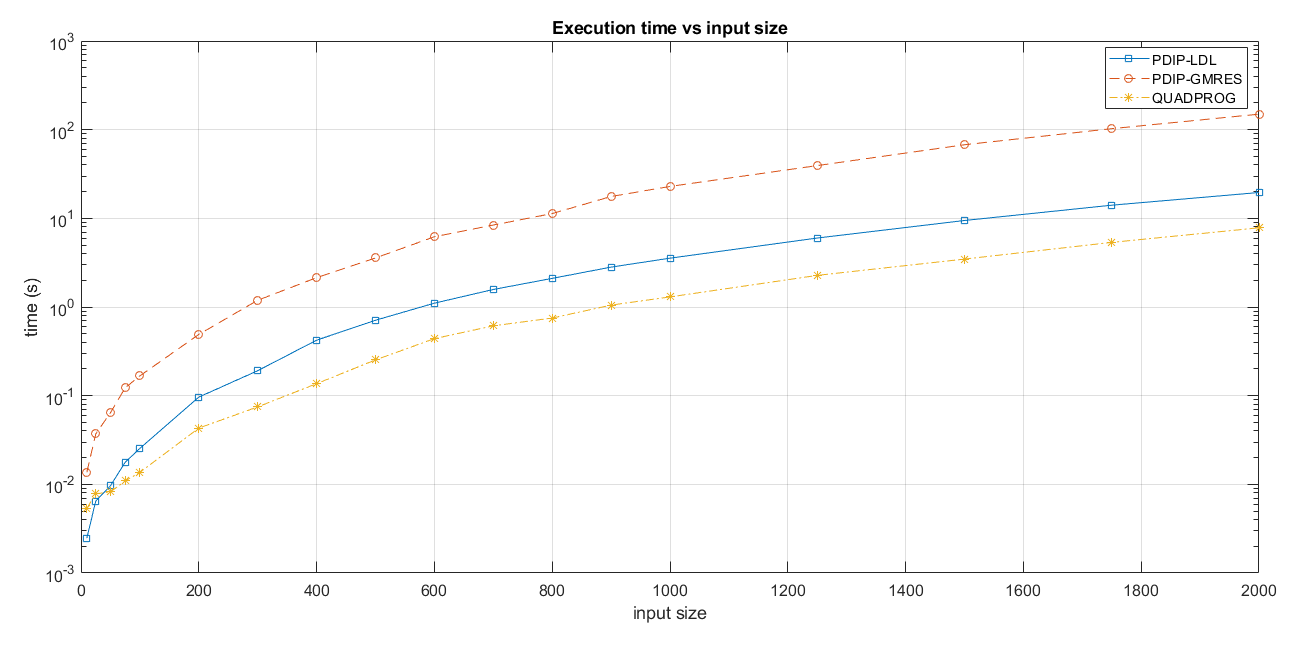
\includegraphics[width=\textwidth]{img/MU1.png}
    \caption{Il grafico mostra l'andamento del tempo di esecuzione (in \textit{log-scale} sulle y) all'aumentare della dimensione del problema. \label{fig:exp1}}
\end{figure}

bhe che dire grafico bellissimo ma corna fai cagare, vediamo na tab che è meglio rcosinniurio

\begin{table}[!h]
\centering
\begin{tabular}{|l|c|c|c|c|c|c|c|c|}
\hline \textbf{input size}                  & \textbf{50}  & \textbf{75}  & \textbf{100} & \textbf{200}  & \textbf{300}  & \textbf{400}  & \textbf{500}  & \textbf{600}  \\\hline
\textbf{PDIP-LDL}                    & 0.0064       & 0.0177       & 0.0211       & 0.0575        & 0.1418        & 0.3251        & 0.5271        & 0.8170        \\
\textbf{QUADPROG}                    & 0.0069       & 0.0115       & 0.0137       & 0.0334        & 0.0737        & 0.1377        & 0.2590        & 0.4541        \\
\textbf{slowfactor} & 0.9259       & 1.5432       & 1.5422       & 1.7229        & 1.9247        & 2.3617        & 2.0351        & 1.7989        \\ \hline
\textbf{input size}                  & \textbf{700} & \textbf{800} & \textbf{900} & \textbf{1000} & \textbf{1250} & \textbf{1500} & \textbf{1750} & \textbf{2000} \\\hline
\textbf{PDIP-LDL}                    & 1.1532       & 1.4939       & 2.0655       & 2.5441        & 4.2911        & 6.8573        & 8.8513        & 11.7768       \\
\textbf{QUADPROG}                    & 0.6157       & 0.7584       & 1.0631       & 1.3172        & 2.2816        & 3.5041        & 5.3935        & 7.9170        \\
\textbf{\textit{slowfactor}} & 1.8728       & 1.9697       & 1.9428       & 1.9315        & 1.8808        & 1.9569        & 1.6411        & 1.4875  \\\hline     
\end{tabular}
    \caption{Tabelle contenenti la media dei tempi di esecuzione (s) di PDIP-LDL e QUADPROG relativi al primo sotto-esperimento. \label{tab:ldlqp2}}
    \end{table}
   
 Risultati brutti, ma veramente name. da fare schifo vediamo altra merda. Grande corna non cambiare mai, la prossima relazione la scrivi tutta te
    
\begin{table}[!h]
\centering
\begin{tabular}{|l|c|c|c|c|c|c|c|c|}\hline
\textbf{input size} & \textbf{50}  & \textbf{75}  & \textbf{100} & \textbf{200}  & \textbf{300}  & \textbf{400}  & \textbf{500}  & \textbf{600}  \\\hline
\textbf{PDIP-LDL}   & 10.65\%      & 29.22\%      & 17.34\%      & 5.81\%        & 8.03\%        & 3.87\%        & 5.03\%        & 1.80\%        \\
\textbf{QUADPROG}   & 13.35\%      & 25.80\%      & 17.72\%      & 2.55\%        & 3.12\%        & 4.95\%        & 19.12\%       & 7.99\%        \\\hline
\textbf{input size} & \textbf{700} & \textbf{800} & \textbf{900} & \textbf{1000} & \textbf{1250} & \textbf{1500} & \textbf{1750} & \textbf{2000} \\\hline
\textbf{PDIP-LDL}   & 3.96\%       & 2.74\%       & 1.67\%       & 1.94\%        & 2.27\%        & 1.56\%        & 2.31\%        & 2.41\%        \\
\textbf{QUADPROG}   & 2.94\%       & 1.37\%       & 1.42\%       & 0.94\%        & 1.13\%        & 0.85\%        & 0.92\%        & 0.83\%     \\  \hline
\end{tabular}
    \caption{Tabella contenente la deviazione standard dei tempi di esecuzione di PDIP-LDL e QUADPROG relativi al primo sotto-esperimento. \label{tab:ldlqp1.1}}
\end{table}


\subsection*{subexp 2}

wewewewewe

\begin{figure}[!h]
    \centering
    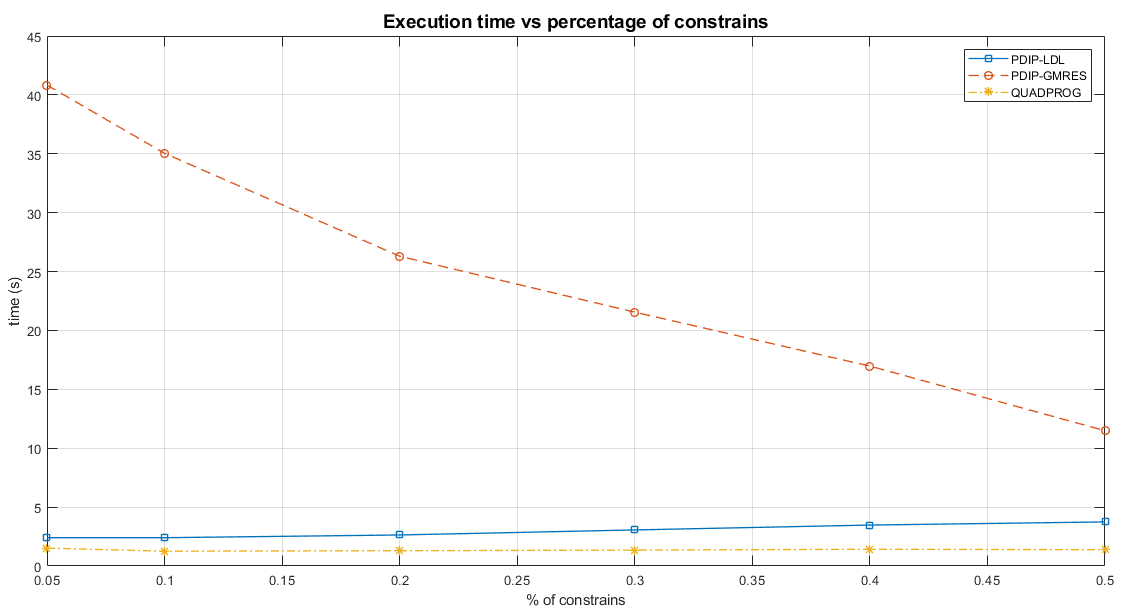
\includegraphics[width=\textwidth, height=7.5cm]{img/MU2.png}
    \caption{Il grafico mostra l'andamento del tempo di esecuzione all'aumentare del numero dei vincoli in $A$. \label{fig:exp1}}
\end{figure}
 
 sembra andare tutto bene,ma guardando quella di dopo possimao notare che facciamo un po' ridere
 
\begin{figure}[!h]
    \centering
    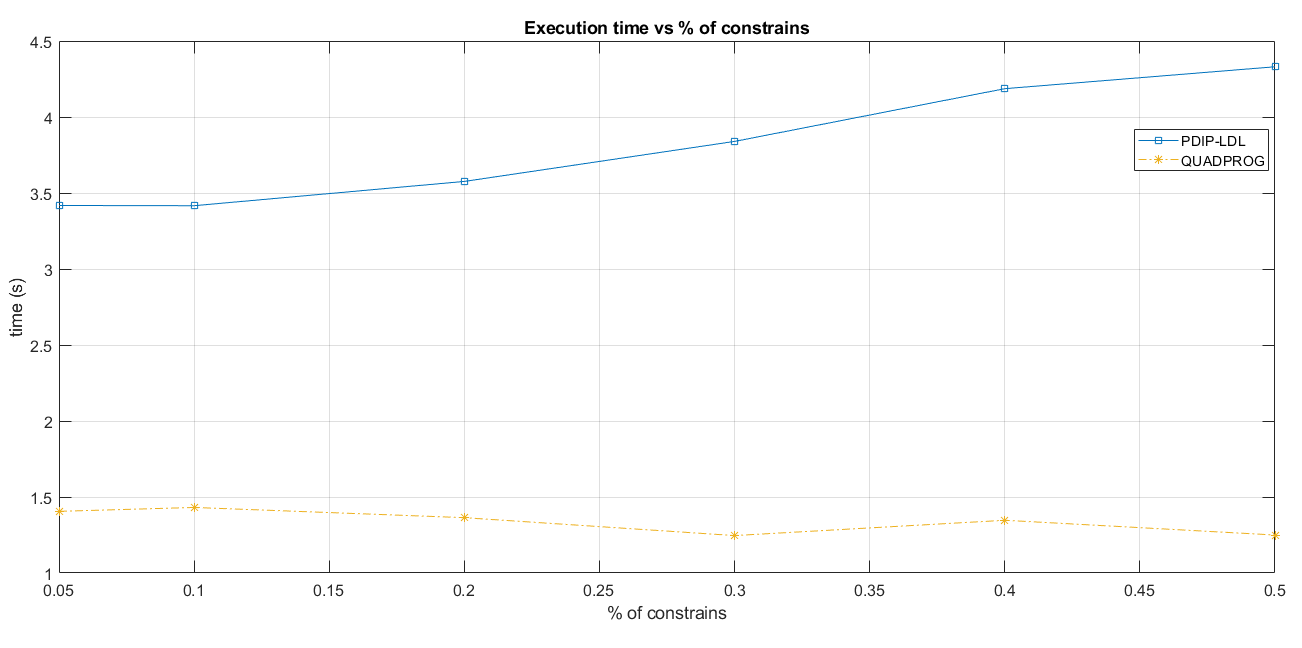
\includegraphics[width=\textwidth, height=7cm]{img/MU3.png}
    \caption{Grafico di confronto fra PIDP-LDL e QUDPROG. \label{fig:exp1.1}}
\end{figure}

e torniamo alle soliute tabelle di me, grande corna

\begin{table}[!h]
\centering
\begin{tabular}{l|c|c|c|c|c|c}

$\mathbf{k/n}$            & \textbf{0.05} & \textbf{0.1} & \textbf{0.2} & \textbf{0.3} & \textbf{0.4} & \textbf{0.5} \\ \hline
\textbf{PDIP-LDL}                    & $2.401 \pm 2.6\%$       & $2.403 \pm 1.8\%$       & $2.634     \pm 2\%$   & $3.062 \pm 3\%$      & $3.476 \pm 1.9\%$      & $3.743 \pm 2.8\%$       \\
\textbf{QUADPROG}                    & $1.519 \pm 3.3\%$       & $1.256 \pm 2.4\%$       & $1.299 \pm 0.9\%$       & $1.351 \pm 1.6\%$       & $1.420 \pm 0.9\%$       & $1.382 \pm 3.6\%$       \\
\textbf{\textit{slowfactor}} & 1.581        & 1.913       & 2.027       & 2.267       & 2.446       & 2.707 
\end{tabular}
\caption{Tabella contenente media e deviazione standard dei tempi di esecuzione (s) di PDIP-LDL e QUADPROG relativi al secondo sotto-esperimento.\label{tab:ldlqp2}}
\end{table}

\subsection*{subexp 3}

molto bello il numero uno al mondo almeno $\leq$

\begin{figure}[h]
    \centering
    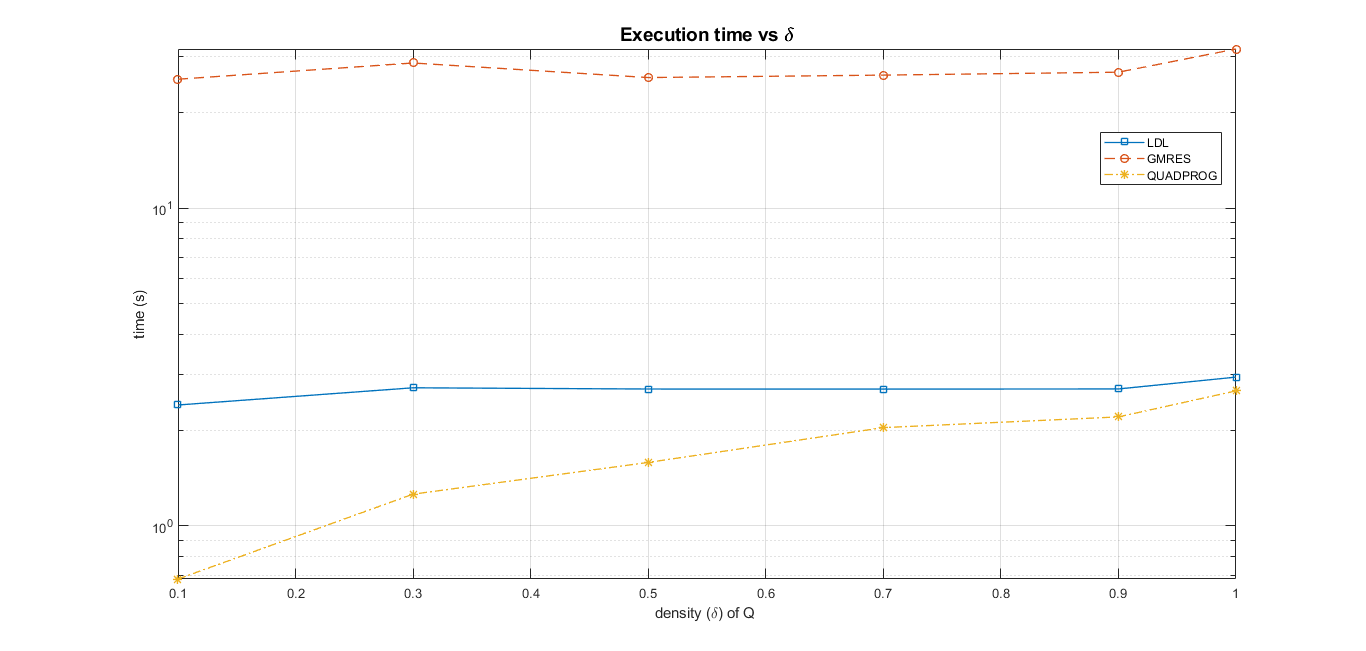
\includegraphics[width=\textwidth]{img/MU4.png}
    \caption{Il grafico mostra l'andamento del tempo di esecuzione (in \textit{log-scale} sulle y) all'aumentare del numero della densità di $Q$. \label{fig:exp1}}
\end{figure}
 


\begin{table}[!h]
\centering
\begin{tabular}{l|c|c|c|c|c|c}
\textbf{density}                     & \textbf{0.1} & \textbf{0.3} & \textbf{0.5} & \textbf{0.7} & \textbf{0.9} & \textbf{1.0} \\ \hline
\textbf{PDIP-LDL}                    & $2.401 \pm 1.2\%$       & $2.719 \pm 2.8\%$       & $2.695  \pm 2\%$       & $2.694 \pm 2.2\%$       & $2.696 \pm 2.3\%$       & $2.938  \pm 2.4\%$       \\
\textbf{QUADPROG}                    & $0.681  \pm 2.2\%$      & $1.258  \pm 5\%$       & $1.583 \pm 2.8\%$       & $2.038 \pm 1.5\%$       & $2.202 \pm 1.1\%$       & $2.659 \pm 5.9\%$       \\
\textbf{\textit{slowfactor}} & 3.526       & 2.161       & 1.701       & 1.321       & 1.224       & 1.104
\end{tabular}
\caption{Tabella contenente media e deviazione standard dei tempi di esecuzione (s) di PDIP-LDL e QUADPROG relativi al terzo sotto-esperimento. \label{tab:ldlqp3}}
\end{table}


\subsection*{Convergenza e Accuratezza della Soluzione}

Qui ci andrebbe il grafico del gap 

\begin{figure}[h]
    \centering
    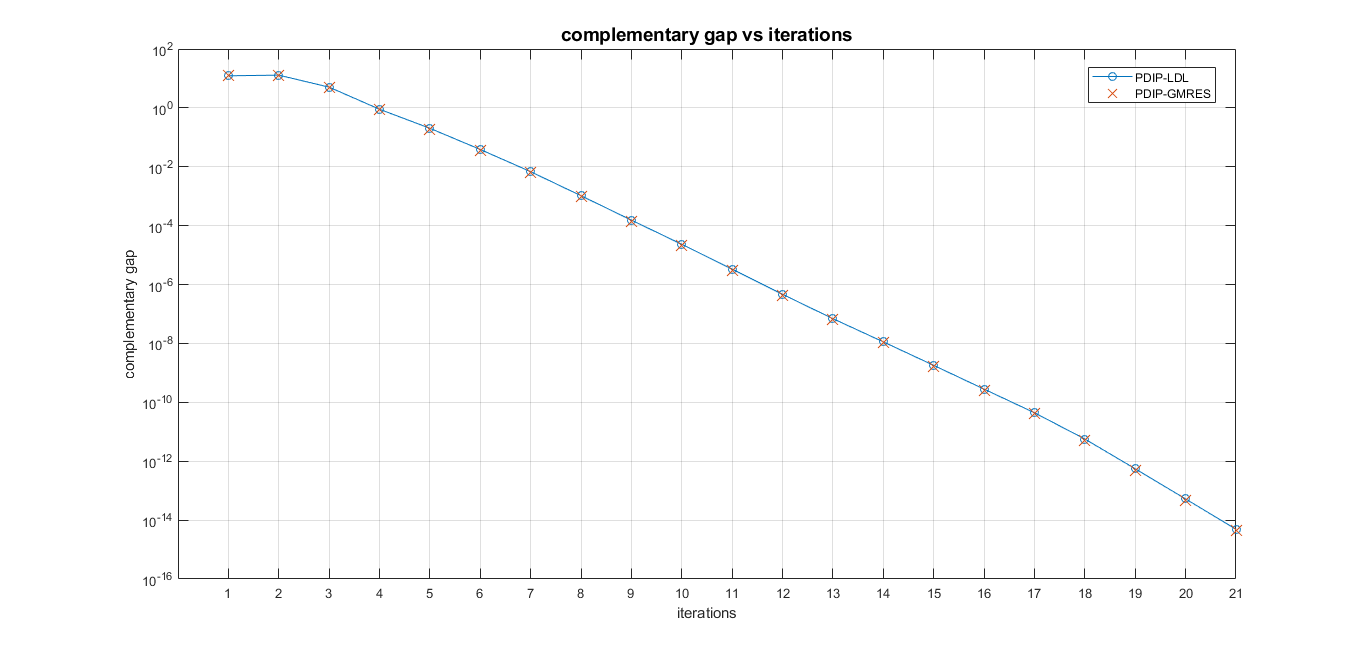
\includegraphics[width=\textwidth]{img/MU6.png}
    \caption{Il grafico mostra l'andamento del gap (in \textit{log-scale} sulle y) all'aumentare delle iterazioni. \label{fig:gap}}
\end{figure}

e magari o una tabella o un grafico con
$$ \norm{x_{LDL} - x_{QUADPROG}} $$
$$ \norm{\nabla L_{LDL} - \nabla L_{QUADPROG}} $$
$$ \norm{\lambda_{LDL} - \lambda_{QUADPROG}} $$

o altro